%!TEX root = paper.tex
%%%%%%%%%%%%%%%%%%%%%%%%%%%%%%%%%%%%%%%%%%%%%%%%%%%%%%%%%%%%%%%%%%%%%%%%%%%%%%%
\section{Supply-Side Efficiency Modeling}
\label{sec:suppliermodelling}

This section assesses the supply-side of the cloud gaming market with a strong focus on costs. The remainder of this section first clarifies typical cost factors in the cloud gaming market and then continues with a specific efficiency model formulation that responds to the demand-side findings of previous sections.

%%%%%%%%%%%%%%%%%%%%%%%%%%%%%%%%%%%%%%%%%%%%%%%%%%%%%%%%%%%%%%%%%%%%%%%%%%%%%%%%
\subsection{Cost Factors}

The dominating cost factor in cloud gaming is the server infrastructure, both in terms of \gls{CAPEX} and \gls{OPEX}. The low latency requirements of many games requires a regionally-oriented cloud infrastructure, i.e., regional data centers are used to provide high-quality and low-latency service. Due to the specific demands of games, specialized hardware is used (e.g., with GPU-enabled CPUs), rather than generic cloud servers. These factors increase the \gls{CAPEX} for cloud service operators, but also lower the efficiency of the system, as more generic and more globalized cloud services cloud yield scaling advantages. Moreover, the rental of generic cloud service hardware or resources seems to be unrealistic due to the lowered efficiency --- cloud services are typically data-centric, while gaming is graphics-intense. The \gls{OPEX} is limited to maintenance activities, consumables, Internet access fees and energy.

In addition, game license fees have to be considered as noteworthy \gls{CAPEX} (or potentially also \gls{OPEX}, depending on the license models). Depending on the licensing model, a flat license (one-time price for an unlimited number of subscribers), volume licenses, or per-use or per usage fees may be arranged with license owners. In all cases, scaling effects probably exist: the initial \gls{CAPEX} is high in terms of license arrangement costs and initial fees, while marginal costs decrease for additional subscribers.

On the customer-side, the subscription or per-game prices represent costs that create the revenue for the cloud gaming provider and for the game license owners. Customers typically also require specific gaming hardware to connect to the platform, which can be cheaper than high-end gaming hardware, but may lower the added value over hardware-intensive conventional gaming approaches.


%%%%%%%%%%%%%%%%%%%%%%%%%%%%%%%%%%%%%%%%%%%%%%%%%%%%%%%%%%%%%%%%%%%%%%%%%%%%%%%%
\subsection{Model}

Based on the collected consumer price figures, this section will elaborate on the required computational efficiency, i.e., cost per hosted subscriber, in order to successfully establish cloud gaming approaches on the market. Due to the limited available data, this investigation will follow a single data center assumption. Due to the demands of cloud gaming to serve both at high performance and low latency, regional data centers will play a dominant role in the provider side cost modeling. Following this assumption, hereinafter a specific model is created that characterizes at which cost efficiency levels the cloud gaming business can be operated successfully.

\begin{figure}[!t]
	\centering
	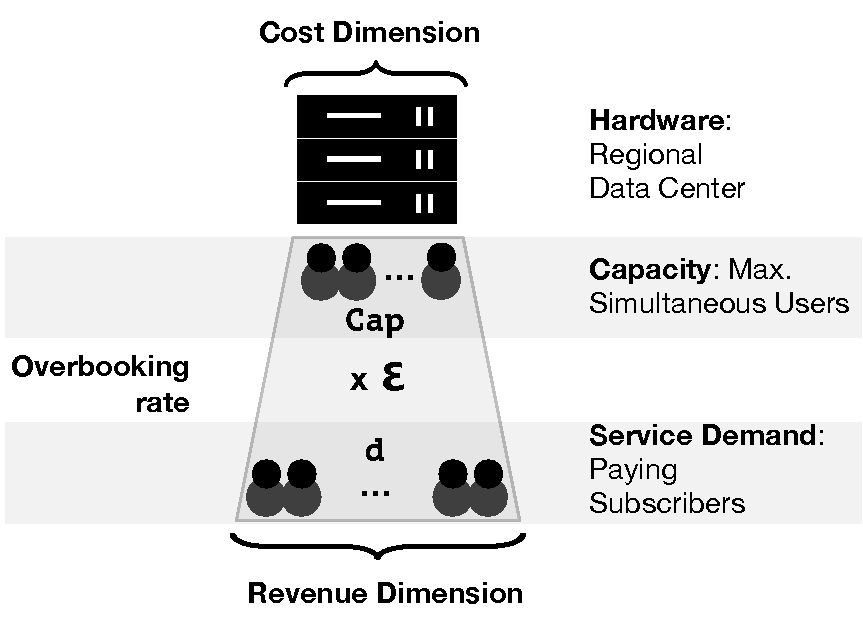
\includegraphics[width=0.75\columnwidth]{images/overbooking_datacenterNG.pdf}
	\caption{Overbooking of available computational capacity.}
\label{fig:overbooking_datacenter}
\end{figure}

The model (Figure~\ref{fig:overbooking_datacenter}) is motivated as follows: a cloud gaming operator must provide a certain data center capacity $Cap$ of slots for the maximum number of gamers that can play simultaneously, so as to provide sufficient availability and quality. This incurs an overall cost of $\mathcal{C}_{Cap}$. Active players recruit from the overall number of subscribers, denoted as the total service demand $d$. In general, not all subscribers will play at the same time. This allows for an overbooking factor $\epsilon$ on the data center resources so that $Cap \cdot \epsilon = d$. The larger the overbooking factor can be made without impacting quality for active players, the smaller the data center capacity may be dimensioned. %, saving costs.
The overall cost must not exceed the average price $\bar{p}$ paid by a subscriber times the the number of subscribers;
scaling this limit to the number of concurrently active users yields the maximum cost per active user $\mathcal{C}_u$ that the operator can spend

\begin{equation}
  \phantom{\text{.}}\mathcal{C}_u = \frac{\mathcal{C}_{Cap}}{Cap} \leq \frac{\bar{p} \cdot d}{Cap} = \frac{\bar{p} \cdot Cap \cdot \epsilon}{Cap} = \bar{p} \cdot \epsilon\text{.}
\end{equation}

To interpret this relationship, estimates for the overbooking factor and average price are discussed. The costs of the regional data center (\gls{CAPEX}, \gls{OPEX}, required game licensing fees) are treated as a black box to simplify the treatment.

A reasonable value for the overbooking factor $\epsilon$ may be derived from the number of active \steam user over the course of two days. As observed\footnote{\url{http://store.steampowered.com/stats/}} between 2016-02-16 and 18, between $6.53$\si{\mega} and $11.65$\si{\mega} users were connected simultaneously. To gain a conservative estimate, the maximum is set in relationship to the $75$ million registered \steam users\footnote{\url{http://venturebeat.com/2014/01/15/steam-has-75-million-registered-users-third-party-steam-controllers-and-other-tidbits-from-valves-dev-days/}}, and calculate an $\epsilon_{\text{Steam}}\approx6.44$. For cross-validation purposes, link load levels for other media streaming services may be considered: When comparing the relative load level change between the minimum and maximum utilization of a large Vietnamese \acrshort{ISP}'s \gls{VoD} streaming server as given in \cite{thanh2012enabling}, the growth from Steam's minimum to its maximum utilization can be rescaled accordingly. A maximum number of simultaneously connected \gls{VoD} users of $58.3$ million and an $\epsilon_{\text{sub}}$ of $1.29$ are obtained. The discrepancy in overbooking factors may appear high, but the different associated payment modalities may be at cause: While \steam sells game licenses (of which the buyer may make use any time), \gls{VoD} services often use a subscription services (a flat rate for a given time period). For the subsequent analysis the range between the minimum of $\epsilon_{\text{sub}}$ and maximum of $\epsilon_{\text{Steam}}$ is considered.

The average price $\bar{p}$ is also parameterized on the basis of the collected \steam data. To reflect the range of the data (see Tbl.~\ref{tab:steam-price-stats}), the minimum and the maximum values are used as inputs for the subsequent cost considerations: $\bar{p}_{\text{min}} = 5.30$, $\bar{p}_{\text{max}} = 12.39$. (For comparison, the monthly subscription rate for \psnow UK is roughly \SI{16.53}[\EUR]{}.)

Lastly (but ignored in the model), the operator may expect a profit margin of \SI{3}{\percent}\footnote{\url{http://www.polygon.com/2012/10/1/3439738/the-state-of-games-state-of-aaa}} to \SI{16.9}{\percent}\footnote{\url{http://www.forbes.com/sites/georgeanders/2015/04/23/amazons-web-services-delight-16-9-margins-more-joy-ahead/\#73324aa64b4e}} (or even higher\footnote{\url{http://www.bloomberg.com/news/articles/2015-12-02/microsoft-should-disclose-cloud-revenue-margins-ballmer-says}}). Requiring a higher profit margin transitively lowers the maximum cost per active user that the operator can tolerate.

Applying the different mean prices and $\epsilon$ values, it can be inferred that the monthly capacity and licensing cost per peak time user $\mathcal{C}_u$ must not exceed $\epsilon_{\text{sub}} \cdot \bar{p}_{\text{min}} = \SI{6.81}[\EUR]{}$ (lower bound scenario) to $\epsilon_{\text{Steam}} \cdot \bar{p}_{\text{max}} = \SI{79.80}[\EUR]{}$, both excluding a profit margin. Scaling these costs to \steam's peak time population of $11.65\si{\mega}$ yields ranges for the maximum allowable server capacity costs $\mathcal{C}_{\text{Cap}}$ per month of \SI{79.4}[\EUR]{M} to \SI{929.3}[\EUR]{M} for a cloud game service of the size of \steam.

In that respect, cost optimizations beside the classical capacity dimensioning also deserve attention. Due to the requirement of using special gaming equipment, however, sharing hardware with other cloud applications seems unrealistic. Thus $\mathcal{C}_u$ can hardly be reduced by cloud service collaboration. However, to lower the investment demands, the platform operator could aim at increasing the overbooking ratio $\epsilon_{sub}$ for the subscription case closer to the $\epsilon_{steam}$ of the classical purchasing model. The provider could, for example, offer off-peak subscriptions that allow the access to the platform only outside of peak hours.

Furthermore, the maximum per-user cost figures do not consider that the operator may not be able to fully utilize the available capacity or may not hold the optimal game licenses at all times. Thus, in practice, target $\mathcal{C}_{u}$ values should be lower than the calculated values.

Nevertheless, this cost perspective still points to an interesting observation: the low $\epsilon_{sub}$ requires a data center capacity closer to the total service demand. Thus, subscription-based cloud gaming approaches have a higher cost pressure than in the case of a more conventional game sales approach ($\epsilon_{steam}$). When setting the cost perspective in relationship to the product offers, the business challenges of cloud-based game providers become apparent. In particular, the high cost pressures seem to lead to a tightly curated game offering approach --- i.e., a small number of offerings (see Figure~\ref{fig:rel-combinedlength-owners}), good overall scores (see Figure~\ref{fig:scores-by-platform}) --- where only economically attractive games can be offered for subscription plans. This is very likely caused by the underlying scale-oriented licensing practices that favor high volumes --- i.e., the initial \gls{CAPEX} is high, but the marginal cost decrease afterwards (Update note 2020: This cost modality may have changed over time. We recommend considering models will distinct entrances barriers for new games). The limited game offering for cloud-based services, as a result of cost factors and limited scaling advantages on the hardware side, however, reduces the utility for the customer, which should lower their willingness-to-pay. Obviously, this induces a particularly challenging business environment in which operators go out of business on a regular basis. This further explains why cloud gaming has remained a small niche despite the high interest by industry, research and probably also customers (Update note 2020: It will remain to be seen, if the second wave of cloud gaming platform will use a different licensing scheme or may profit from technical scalability advancements that may generate better prospects than for the first wave of platforms).
